\subsection{A-模的复形}

定义 1. --- A-模的微分复形是一个对 (C, d)，由分次 A-模 C 和一个按降次 -1 分级的自同态 \(d: \mathbf{C} \to \mathbf{C}\) 组成，并且使得 \(d \circ d = 0\) 。

它也被称为A-模复形，或A-复形，或简称为复形。人们常将(C, d)简写为C；自同态d被称为复形(C, d)的微分，或者，在不严格的说法中，称为C的微分。

若 \(C_{n}\) (相应地， \(C^{n}\) ）是C的下降（相应地，上升）次数n的齐次分量，d的数据等价于同态序列

\[
\dots \longrightarrow \mathrm{C} _ {n + 1} \xrightarrow {d _ {n + 1}} \mathrm{C} _ {n} \xrightarrow {d _ {n}} \mathrm{C} _ {n - 1} \longrightarrow \dots\tag{1}
\]

分别

\[
\dots \longrightarrow \mathrm{C} ^ {n - 1} \xrightarrow {d ^ {n - 1}} \mathrm{C} ^ {n} \xrightarrow {d ^ {n}} \mathrm{C} ^ {n + 1} \longrightarrow \dots\tag{1'}
\]

使得 \(d_n \circ d_{n+1} = 0\) 对所有 \(n \in \mathbf{Z}\) 成立（相应地， \(d^n \circ d^{n-1} = 0\) 对所有 \(n \in \mathbf{Z}\) 成立）。按语言滥用，这样的A-模与同态序列的数据也将被称为复形。

作为助记，注意在图表（1）和（1'）中“沿箭头方向”时，下降的次数递减，上升的次数递增。

每个分次 A-模都将默认通过赋予其零微分而视为一个复形；如此得到的复形将被称为具有零微分的复形。特别地，每个 A-模 M 都将被赋予唯一的 A-复形结构，使得 \(M_{0} = M^{0} = M\) 。复形 (C, d) 称为零复形，如果 C 化归为 0。在下文中，我们用 0 表示一个一次性选定的零复形。

让我们在有序集 Z 上添加两个元素，记为 \(-\infty\) 和 \(+\infty\) ；记 \(\overline{Z}\) 为所得到的集合，并赋予它一个序关系，该序关系扩展了 Z 上的序关系，且使得 \(-\infty < n < +\infty\) 对所有 \(n \in Z\) 成立；\(\overline{Z}\) 的每个子集都有下界和上界。

设 C 是一个复形；其右界和左界 \(^{1}\) 是元素 \(b_{d}(\mathbf{C})\) 和 \(b_{g}(\mathbf{C})\) （属于 \(\overline{\mathbf{Z}}\) ），定义如下

\[
b _ {d} (\mathbf {C}) = \inf \left\{n \in \mathbf {Z}, \mathrm{C} _ {n} \neq 0 \right\}, \quad b _ {g} (\mathbf {C}) = \sup \left\{n \in \mathbf {Z}, \mathrm{C} _ {n} \neq 0 \right\}.
\]

称 C 在右侧为零，如果 \(b_{d}(\mathbf{C}) \geqslant 0\) ，在右侧有界，如果 \(b_{d}(\mathbf{C}) \neq -\infty\) ，在左侧为零，如果 \(b_{g}(\mathbf{C}) \leqslant 0\) ，在左侧有界，如果 \(b_{g}(\mathbf{C}) \neq +\infty\) ；称 C 是有界的，如果

\[
b _ {d} (\mathbf {C}) \neq - \infty , \quad b _ {g} (\mathbf {C}) \neq + \infty .
\]

长度 \(^{2}\) ，记为 \(l(\mathbf{C})\)，是 \(\overline{\mathbf{Z}}\) 的元素，定义如下：若 C 为零，则 \(l(\mathbf{C}) = -\infty\) ；若 C 有界且非零，则 \(l(\mathbf{C}) = b_{g}(\mathbf{C}) - b_{d}(\mathbf{C})\) ；若 C 无界，则 \(l(\mathbf{C}) = +\infty\) 。* 按照 TG, IV, p.～13-17 的约定，总有 \(l(\mathbf{C}) = b_{g}(\mathbf{C}) - b_{d}(\mathbf{C})\) 。*

例如，如果 \(k\) 个相邻的 \(C\) 的分量非零而其余的为零，则我们有 \(l(C) = k - 1\) （如果 \(k > 0\) ），以及 \(l(C) = -\infty\) （如果 \(k = 0\) ）。

我们说复形(C, d)是自由的、投射的、平坦的、内射的，如果每个模 \(C_{n}\) 确实如此。注意，复形 (C, d) 是投射的或平坦的，当且仅当模 C 是（II，第 39 页，命题 3 及 X，第 8 页，命题 4），但 C 可以是自由的，而复形 (C, d) 却不是（因为自由模的直和因子不总是自由的），正如 (C, d) 可以是内射的，而 C 却不是（X，第 170 页，习题 21）。

\pandocbounded{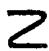
\includegraphics[keepaspectratio]{images/part001_579990b7.jpg}}

设 (C, d) 为一个复形。我们令 \(\mathbf{Z}(\mathbf{C}, d) = \operatorname{Ker}(d)\) , \(\mathbf{B}(\mathbf{C}, d) = \operatorname{Im}(d)\) ，它们是 C 的分次子模，分别称为 (C, d) 的闭链模和边缘模；\(\mathbf{Z}(\mathbf{C}, d)\) 和 \(\mathbf{B}(\mathbf{C}, d)\) 的齐次分量被记为 \(\mathbf{Z}_{n}(\mathbf{C}, d) = \mathbf{Z}^{-n}(\mathbf{C}, d)\) , \(\mathbf{B}_{n}(\mathbf{C}, d) = \mathbf{B}^{-n}(\mathbf{C}, d)\) ；我们有 \(\mathbf{Z}_{n}(\mathbf{C}, d) = \operatorname{Ker}(d_{n})\) , \(\mathbf{B}_{n}(\mathbf{C}, d) = \operatorname{Im}(d_{n+1})\) , \(\mathbf{Z}^{n}(\mathbf{C}, d) = \operatorname{Ker}(d^{n})\) , \(\mathbf{B}^{n}(\mathbf{C}, d) = \operatorname{Im}(d^{n-1})\) .

由于 \(d \circ d = 0\) ，我们有 \(\mathrm{B}(\mathrm{C}) \subset \mathrm{Z}(\mathrm{C})\) ；两个闭链若其差为一个边缘，则称它们是同调的；商分次模 \(\mathrm{H}(\mathrm{C}, d) = \mathrm{Z}(\mathrm{C}, d)/\mathrm{B}(\mathrm{C}, d)\) 被称为 \((\mathrm{C}, d)\) 的同调模；其元素是同调类；其齐次分量记为 \(\mathrm{H}_n(\mathrm{C}, d) = \mathrm{H}^{-n}(\mathrm{C}, d)\) 。

例。--- 若 C 的微分为零，则有 \(Z(C) = C\) , \(B(C) = 0\) ，且 \(H(C)\) 典范地等同于 \(C\) 。

我们有正合序列，称为典范的：

\((I_{n})\)

\[
0 \longrightarrow \mathrm{Z} _ {n} (\mathrm{C}) \longrightarrow \mathrm{C} _ {n} \stackrel {\delta_ {n}} {\longrightarrow} \mathrm{B} _ {n - 1} (\mathrm{C}) \longrightarrow 0\tag{\((\mathrm{II}_{n})\)}
\]

\[
0 \longrightarrow \mathrm{B} _ {n} (\mathrm{C}) \longrightarrow \mathrm{Z} _ {n} (\mathrm{C}) \longrightarrow \mathrm{H} _ {n} (\mathrm{C}) \longrightarrow 0
\]

\((\mathrm{III}_{n})\)

\[
0 \longrightarrow \mathrm{B} _ {n} (\mathrm{C}) \longrightarrow \mathrm{C} _ {n} \longrightarrow \mathrm{C} _ {n} / \mathrm{B} _ {n} (\mathrm{C}) \longrightarrow 0
\]

\((\mathrm{IV}_n)\)

\[
0 \longrightarrow \mathrm{H} _ {n} (\mathrm{C}) \longrightarrow \mathrm{C} _ {n} / \mathrm{B} _ {n} (\mathrm{C}) \stackrel {\overline {{\delta}} _ {n}} {\longrightarrow} \mathrm{B} _ {n - 1} (\mathrm{C}) \longrightarrow 0
\]

其中 \(\delta_{n}\) 和 \(\overline{\delta}_{n}\) 由 \(d_{n}\) 推出。通过结合 \((\mathrm{IV}_{n})\) 和 \((\mathrm{II}_{n-1})\) ，得到正合序列

\[
0 \rightarrow \mathrm{H} _ {n} (\mathrm{C}) \rightarrow \mathrm{C} _ {n} / \mathrm{B} _ {n} (\mathrm{C}) \rightarrow \mathrm{Z} _ {n - 1} (\mathrm{C}) \rightarrow \mathrm{H} _ {n - 1} (\mathrm{C}) \rightarrow 0,\tag{\((\mathbf{V}_n)\)}
\]

将 n 换成 -n，也可将它写成

\[
0 \rightarrow \mathrm{H} ^ {n} (\mathrm{C}) \rightarrow \mathrm{C} ^ {n} / \mathrm{B} ^ {n} (\mathrm{C}) \rightarrow \mathrm{Z} ^ {n + 1} (\mathrm{C}) \rightarrow , \mathrm{H} ^ {n + 1} (\mathrm{C}) \rightarrow 0.\tag{\((\mathbf{V}^n)\)}
\]

定义2.——设(C, d)和(C', d')是两个复形。从 (C, d) 到 (C', d') 的态射 \(^{1}\) 是从 C 到 C' 的次数为 0 的分次 A-同态 u，使得

\[
d ^ {\prime} \circ u = u \circ d.
\]

对于每一个 \(n\) ，我们有 \(d_n' \circ u_n = u_{n-1} \circ d_n\) 和 \(d''n \circ u^n = u^{n+1} \circ d^n\) 。我们有

\[
u (\mathbf {Z} (\mathbf {C})) \subset \mathbf {Z} (\mathbf {C} ^ {\prime}), \quad u (\mathbf {B} (\mathbf {C})) \subset \mathbf {B} (\mathbf {C} ^ {\prime}),
\]

并且我们用 \(Z(u):Z(C)\to Z(C')\) , \(B(u):B(C)\to B(C')\) , \(H(u):H(C)\to H(C')\) 表示由它们推出的A-模同态；这些态射的齐次分量记为 \(Z_{n}(u)\) , \(Z^{n}(u)\) , \ldots{}

若 \(v\) 是另一个从 \((\mathbf{C}, d)\) 到 \((\mathbf{C}', d')\) 的态射，则 \(u + v\) 是从 \((\mathbf{C}, d)\) 到 \((\mathbf{C}', d')\) 的态射，并且我们有

\[
\mathbf {Z} (u + v) = \mathbf {Z} (u) + \mathbf {Z} (v), \quad \mathbf {B} (u + v) = \mathbf {B} (u) + \mathbf {B} (v), \quad \mathbf {H} (u + v) = \mathbf {H} (u) + \mathbf {H} (v)
\]

类似地，若A是交换环 \(k\) 上的代数，且如果 \(\lambda \in k\) ，则 \(\lambda u\) 是从 \((C, d)\) 到 \((C', d')\) 的态射，并且我们有

\[
\mathbf {Z} (\lambda u) = \lambda \mathbf {Z} (u), \quad \mathbf {B} (\lambda u) = \lambda \mathbf {B} (u), \quad \mathbf {H} (\lambda u) = \lambda \mathbf {H} (u).
\]

若 \(u': (C', d') \to (C'', d'')\) 是另一个复形态射，则 \(u' \circ u\) 是从 \((C, d)\) 到 \((C'', d'')\) 的态射，并且我们有

\[
\mathrm{Z} \left(u ^ {\prime} \circ u\right) = \mathrm{Z} \left(u ^ {\prime}\right) \circ \mathrm{Z} (u), \quad \mathrm{B} \left(u ^ {\prime} \circ u\right) = \mathrm{B} \left(u ^ {\prime}\right) \circ \mathrm{B} (u), \quad \mathrm{H} \left(u ^ {\prime} \circ u\right) = \mathrm{H} \left(u ^ {\prime}\right) \circ \mathrm{H} (u).
\]

显然，双射态射即同构。

定义3.——设(C, d)和(C', d')是两个复形。从(C, d)到(C', d')的同调态射（或拟同构）是一个从(C, d)到(C', d')的态射u，使得H(u)是双射。

每个同构都是同调态射，并且由同调态射复合而成的任何态射都是同调态射。

称(C, d)具有零同调，若H(C) = 0，即若唯一的复形态射 \(0 \rightarrow C\) （相应地，C → 0）是一个同调态射。称（C, d）在降次数 n（相应地，在升次数 n）上是零调的，如果 \(\mathrm{H}_{n}(\mathrm{C}) = 0\) (相应地， \(\mathrm{H}^{n}(\mathrm{C}) = 0\) ).

设 (C, d) 为一个复形且 \(p \in Z\) ；(C, d) 的第 p 次平移是如下得到的复形 (C(p), d(p))：C(p) 是通过将 C 的分次平移 p 得到的 A-模（II，第 163 页；例 3），因此

\[
\mathrm{C} (p) _ {n} = \mathrm{C} _ {n + p}, \quad \mathrm{C} (p) ^ {n} = \mathrm{C} ^ {n - p};
\]

特别地 \(\mathbf{C}(p)_{0} = \mathbf{C}_{p}\) ；还需注意 C 是其分次子模 \(\mathbf{C}_{p}(-p)\) , \(p \in \mathbf{Z}\) （相应地， \(\mathbf{C}^{p}(p)\) , \(p \in \mathbf{Z}\) ）的直和。定义 \(d(p) = (-1)^{p} d\) 。我们有 \(\mathbf{Z}(\mathbf{C}(p)) = \mathbf{Z}(\mathbf{C})(p)\) , \(\mathbf{B}(\mathbf{C}(p)) = \mathbf{B}(\mathbf{C})(p)\) 和 \(\mathrm{H}(\mathbf{C}(p)) = \mathrm{H}(\mathbf{C})(p)\) 。

例如， \(d\) 是从 C 到 C(-1) 的复形态射，并且

\[
\mathrm{H} (d): \mathrm{H} (\mathbf {C}) \to \mathrm{H} (\mathbf {C}) (- 1)
\]

是零。

对于每个复形态射 \(u:(\mathbf{C},d)\to(\mathbf{C}^{\prime},d^{\prime})\) ，以及每个 \(p\in\mathbf{Z}\) , \(u\) 也是从 \((\mathbf{C}(p),d(p))\) 到 \((\mathbf{C}^{\prime}(p),d^{\prime}(p))\) 的态射；它有时被记为 \(u(p)\) 并且我们有

\[
u (p) _ {n} = u _ {n + p}, \quad u (p) ^ {n} = u ^ {n - p}.
\]
% semantic-fragments: legacy-input-seam
\relax{}
